\section{什么是计算机科学}


计算机科学不好定义,由于在名字中有“计算机”一词。然而,计算机科学并非简单地研究计算机,尽管计算机作为一种工具在学科中发挥重要的支持作用,但它们只是工具。


计算机科学研究问题、解决问题并生成解决问题的方案。给定一个问题,计算机科学家的目标是开发一个算法,一系列的指令列表,用于解决可能出现的问题。算法遵循它有限的过程就可以解决问题。


计算机科学可以被认为是对算法的研究。但是,我们必须清楚地认识到,一些问题可能没有解决方案。虽然证明这种说法正确性超出了本文的范围,但一些问题不能解决的事实对于那些研究计算机科学的人是很重要的。可以这么说,计算机科学研究有解决方案和没有解决方案的问题。


当描述问题及其解决方案时,会提到计算一词。若存在一个算法解决某个问题,就称该问题是可计算的。计算机科学的另一个定义是:计算机科学是研究那些可计算和不可计算的问题,研究是不是存在一种算法来解决它。请注意这里没有涉及到“计算机”一词,解决方案与机器无关。


计算机科学,因涉及问题解决过程本身,是关于抽象的研究。抽象使我们能从逻辑视角和物理视角来分别看待问题及解决方案。基本思想跟我们常见的例子一样。


假设你开车上学或上班。作为司机,也就是汽车的用户,你为了让汽车载你到目的地,你会和汽车有些互动,如上汽车、插钥匙、点火、换挡、制动、加速和转向。从抽象的角度,你所看到的是汽车的逻辑视角。你使用的是汽车设计者提供的功能,将你从一个地方载到另一个地方。这些功能有时也被称为接口。


另一方面,汽车修理师傅则有一个截然不同的视角。他不仅知道如何开车,还必须知道所有必要的细节,使我们认为理所当然的功能运行起来。他需要了解发动机如何工作、变速箱如何变速、温度如何控制等等。这就是物理视角,细节发生在“引擎盖下”。


我们用电脑时也会发生同样的情况。大多数人使用计算机写文档、收发电子邮件、上网冲浪、播放音乐、存储图像和玩游戏,但他们并不知道这些应用程序工作的细节。他们从逻辑或用户角度看待计算机。计算机科学家、程序员、技术支持人员和系统管理员看待计算机的角度截然不同。他们必须知道操作系统如何工作、如何配置网络协议以及如何编写控制功能的各种脚本。总言之,他们必须能够控制底层的细节。



这两个例子的共同点是用户态的抽象,也称为客户端,不需要知道细节,只要用户知道接口的工作方式。这个接口是用户与底层沟通的方式。作为抽象的另一个例子,Python 数学模块。一旦导入模块,我们可以执行计算
\begin{lstlisting}
  >>> import math
  >>> math.sqrt(16)
  4.0
  >>>
\end{lstlisting}


这是一个抽象的例子。我们没必要知道如何计算平方根,只需知道函数是什么以及如何使用它。如果导入正确,我们就认为函数会提供正确的结果。我们知道,有人实现了平方根问题的解决方案,但我们只需知道如何去使用它。这是一个“黑盒子”,其接口可描述为:函数名、参数、返回值,其细节隐藏在内部:
\begin{figure}[htbp]
  \centering
  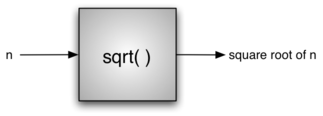
\includegraphics[width=3in]{images/blackbox.png}
\end{figure}
